% Generated from paper/source. Do not edit by hand.
\section{Architecture}
\subsection{Evidence representation}
NeuroWorld emits 40 binary findings, demographic context, explicit observation masks, and an observed sequence. A positive observation and a negative observation use distinct token identities; a missing finding supplies no token. Each token carries normalized time and may be accompanied by a context-conditioned injection. This representation prevents the common leakage-prone shortcut of coding “not observed” as “observed absent.” Unordered baselines receive the same information content through separate positive, negative, and missing channels, but not the chronology needed to solve order twins.

The complex operator state uses a learned initial vector, evidence embeddings, evidence-specific diagonal actions, and factorized low-rank transformations. Low-rank factors keep the parameter count near 20,000 real scalars, comparable to the small baselines. The real operator uses the same sequence interface. The two-channel real model receives paired state channels and a quadratic readout so that extra width and squared measurement are not mistaken for a uniquely complex effect.

\subsection{Conventional controls}
The comparison suite includes logistic regression, an unordered MLP, a tiny Transformer, a validation-tuned GRU, and a diagonal state-space model. Logistic regression and the MLP establish performance available from aggregated evidence. The Transformer tests attention over observed order at a similar scale. The GRU supplies a strong recurrent inductive bias and is tuned only on source validation NLL. The diagonal state-space model tests compact linear recurrence with learned input and nonlinear readout.

The full-data chronology task saturates for all ordered controls, so it is treated as a correctness check. The low-data and shifted worlds carry the architectural comparison. This distinction was introduced after the original baseline set proved too weak: the tuned GRU reverses the apparent source-world sample-efficiency advantage of the operator models, while becoming fragile under generator shift. Preserving that reversal is central to the architecture story.

\subsection{Mechanism families}
Eighteen laws are evaluated in the broad mechanism suite. In addition to the conventional and operator models, these include a complex MLP, modern-Hopfield-style retrieval, a declared factor-graph network, a multiplicative coupled-tensor model, energy and adaptive attractors, Hamiltonian-style evolution, elementwise dissipation, their hybrid, and low-rank density dynamics. The graph control uses the simulator’s coarse factor grouping but not label-specific causal probabilities; its poor result warns that broad causal alignment is not equivalent to learning the generator.

Associative and attractor models intentionally sum or pool evidence before iterative inference, so failure on chronology pairs is expected. That failure is useful: it verifies that the counterfactual task reacts to an architectural invariance rather than merely rewarding model size. Hamiltonian and complex operator laws retain order. Density dynamics also retain a sequential state, but its diagnosis-space factorization and diagonal measurement create a different ambiguity--robustness compromise.

\begin{figure}[t]
\centering
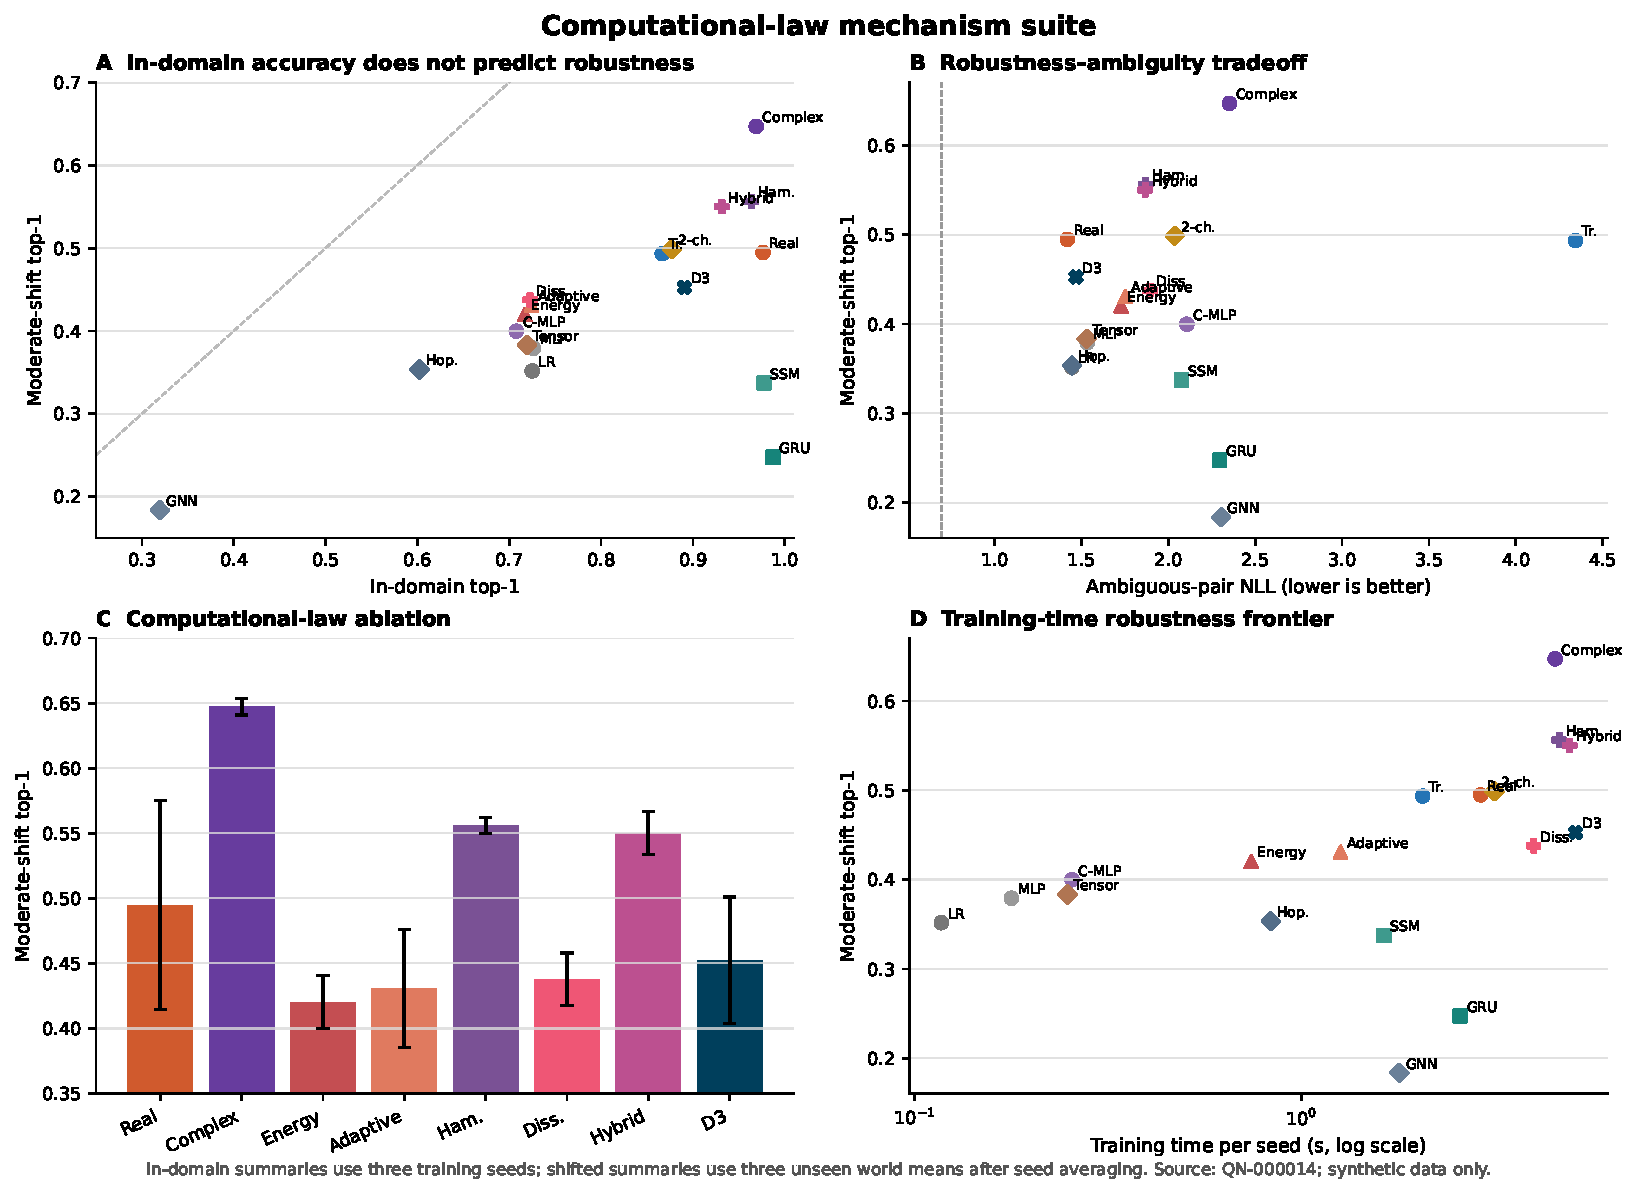
\includegraphics[width=0.98\linewidth]{figures/dynamics_suite.pdf}
\caption{Eighteen computational laws occupy different positions in source accuracy, unseen-world robustness, ambiguity, and chronology-pair performance. No single family dominates every objective.}
\label{fig:dynamics_suite}
\end{figure}

\subsection{Parameter and compute matching}
Most neural architectures are configured near 20,000 trainable real scalars. Complex parameters count as two real scalars. Some controls are smaller by design: logistic regression has 1,660 parameters, while the density model is approximately 16,240. Parameter matching does not imply compute matching. Complex multiplication and evidence-specific operators are slower than the MLP and often slower than the real control on CPU. Training time, process memory, and inference latency are therefore measured separately.

Peak RSS values are interpreted cautiously because sequential in-process runs can reuse allocator caches. Wall-clock times are machine-specific and only compare runs on the same hardware and code path. The public artifacts include environment and configuration records so that external replication can distinguish algorithmic trends from one-machine timing.

\subsection{Architectural invariants}
Unit tests and experiment-time checks enforce that padding does not evolve a state, complex probabilities are finite and normalized, state norms remain bounded, counterfactual pairs differ only in the declared causal factor, and density matrices are Hermitian, positive semidefinite, and unit trace within tolerance. A synthetic nonzero-commutator test confirms that swapping two learned operators can change state. These checks validate implementation properties; they do not show that the learned noncommutativity is causally responsible for every performance difference.

\subsection{Architecture selection after falsification}
The most defensible architectural object at the end of the study is the simple complex operator, not the most elaborate dynamical proposal. Pure Hamiltonian evolution is competitive under shift, but remains below the complex operator. Adding generic dissipation does not help. Increasing density rank does not help. The adaptive attractor does not produce meaningful case-dependent depth. The coupled tensor and graph controls do not approach the robustness frontier. This result argues for retaining the smallest law that survives the declared ablations while treating more ornate mechanisms as negative evidence.

The selected architecture should still not be called “the best model.” The GRU is better at extreme source-world sample efficiency, the real operator is much better on irreducible ambiguity, and several conventional states support stronger linear factor probes. Q-Neuro’s value is conditional: within the tested synthetic family, it combines high chronology accuracy with the strongest moderate-shift top-1 result. Its costs remain visible in every summary.
